\begin{center}
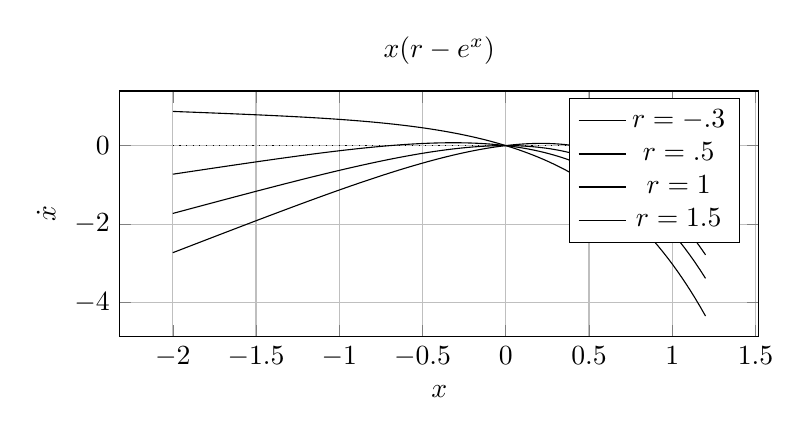
\begin{tikzpicture}
\begin{axis}[width=.8\textwidth,height=4.7cm,xlabel={$x$},ylabel={$\dot x$},title={$x(r-e^x)$},domain=-2:1.2,samples=100,grid=major,legend pos=north east]
\foreach \rr in {-.3,.5,1,1.5}{\addplot[no marks]{x*(\rr-exp(x))};\addlegendentryexpanded{$r=\rr$}}
\addplot[thin,dotted]coordinates{(-2,0)(1.2,0)};
\end{axis}
\end{tikzpicture}

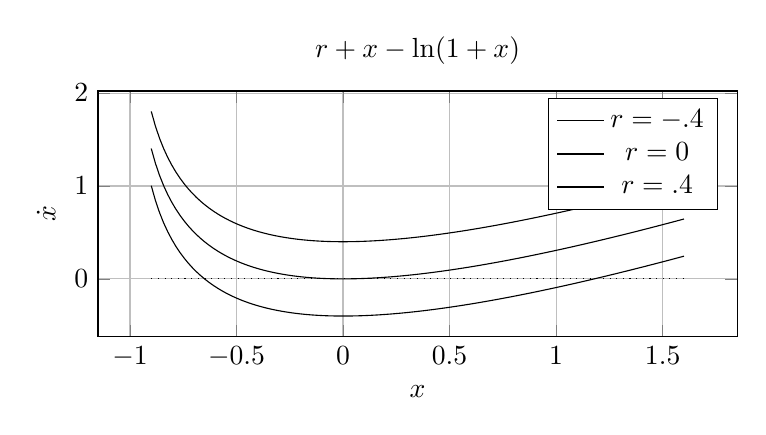
\begin{tikzpicture}
\begin{axis}[width=.8\textwidth,height=4.7cm,xlabel={$x$},ylabel={$\dot x$},title={$r+x-\ln(1+x)$},domain=-.9:1.6,samples=130,grid=major,legend pos=north east]
\foreach \rr in {-.4,0,.4}{\addplot[no marks]{\rr+x-ln(1+x)};\addlegendentryexpanded{$r=\rr$}}
\addplot[thin,dotted]coordinates{(-.9,0)(1.6,0)};
\end{axis}
\end{tikzpicture}

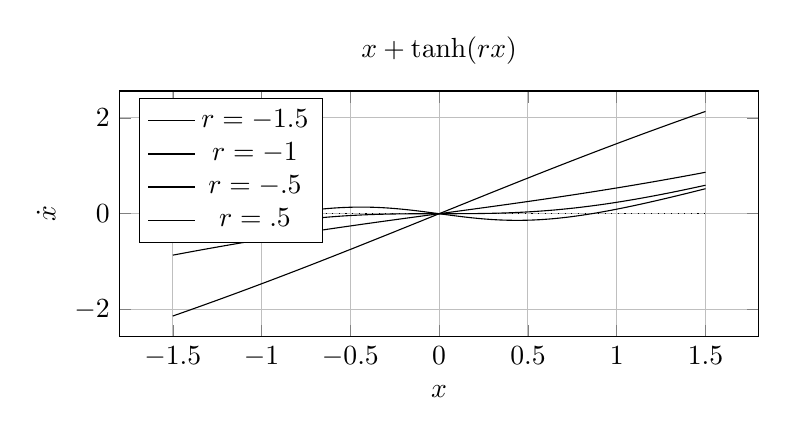
\begin{tikzpicture}
\begin{axis}[width=.8\textwidth,height=4.7cm,xlabel={$x$},ylabel={$\dot x$},title={$x+\tanh(rx)$},domain=-1.5:1.5,samples=120,grid=major,legend pos=north west]
\foreach \rr in {-1.5,-1,-.5,.5}{\addplot[no marks]{x+(exp(2*\rr*x)-1)/(exp(2*\rr*x)+1)};\addlegendentryexpanded{$r=\rr$}}
\addplot[thin,dotted]coordinates{(-1.5,0)(1.5,0)};
\end{axis}
\end{tikzpicture}
\end{center}
三幅是原函数本身的$\dot x$曲线, 与前面的局部分岔示意分开. 曲线在横轴上方表示向右运动, 下方表示向左; 交点是固定点.
